
%% Copernicus Publications Manuscript Preparation Template for LaTeX Submissions
%% ---------------------------------
%% This template should be used for copernicus.cls
%% The class file and some style files are bundled in the Copernicus Latex Package, which can be downloaded from the different journal webpages.
%% For further assistance please contact Copernicus Publications at: production@copernicus.org
%% https://publications.copernicus.org/for_authors/manuscript_preparation.html


%% Please use the following documentclass and journal abbreviations for discussion papers and final revised papers.

%% 2-column papers and discussion papers
\documentclass[journal abbreviation, manuscript]{copernicus}



%% Journal abbreviations (please use the same for discussion papers and final revised papers)


% Advances in Geosciences (adgeo)
% Advances in Radio Science (ars)
% Advances in Science and Research (asr)
% Advances in Statistical Climatology, Meteorology and Oceanography (ascmo)
% Annales Geophysicae (angeo)
% Archives Animal Breeding (aab)
% ASTRA Proceedings (ap)
% Atmospheric Chemistry and Physics (acp)
% Atmospheric Measurement Techniques (amt)
% Biogeosciences (bg)
% Climate of the Past (cp)
% DEUQUA Special Publications (deuquasp)
% Drinking Water Engineering and Science (dwes)
% Earth Surface Dynamics (esurf)
% Earth System Dynamics (esd)
% Earth System Science Data (essd)
% E&G Quaternary Science Journal (egqsj)
% Fossil Record (fr)
% Geochronology (gchron)
% Geographica Helvetica (gh)
% Geoscience Communication (gc)
% Geoscientific Instrumentation, Methods and Data Systems (gi)
% Geoscientific Model Development (gmd)
% History of Geo- and Space Sciences (hgss)
% Hydrology and Earth System Sciences (hess)
% Journal of Micropalaeontology (jm)
% Journal of Sensors and Sensor Systems (jsss)
% Mechanical Sciences (ms)
% Natural Hazards and Earth System Sciences (nhess)
% Nonlinear Processes in Geophysics (npg)
% Ocean Science (os)
% Primate Biology (pb)
% Proceedings of the International Association of Hydrological Sciences (piahs)
% Scientific Drilling (sd)
% SOIL (soil)
% Solid Earth (se)
% The Cryosphere (tc)
% Web Ecology (we)
% Wind Energy Science (wes)


%% \usepackage commands included in the copernicus.cls:
%\usepackage[german, english]{babel}
%\usepackage{tabularx}
%\usepackage{cancel}
%\usepackage{multirow}
%\usepackage{supertabular}
%\usepackage{algorithmic}
%\usepackage{algorithm}
%\usepackage{amsthm}
%\usepackage{float}
%\usepackage{subfig}
%\usepackage{rotating}


\begin{document}

\title{Digital supplement for ``Synergistic radar and sub-millimeter radiometer retrievals of ice clouds''}

% \Author[affil]{given_name}{surname}

\Author[1]{Simon}{Pfreundschuh}
\Author[1]{Patrick}{Eriksson}
\Author[2]{Stefan A.}{Buehler}
\Author[2]{Manfred}{Brath}
\Author[4]{David}{Duncan}
\Author[3]{Richard}{Larsson}
\Author[2]{Robin}{Eklund}

\affil[1]{Department of Space, Earth and Environment, Chalmers University of Technology, 41296 Gothenburg, Sweden}
\affil[2]{Meteorologisches Institut, Fachbereich Geowissenschaften, Centrum für Erdsystem und Nachhaltigkeitsforschung (CEN), Universität Hamburg, Bundesstraße 55, 20146 Hamburg, Germany}
\affil[3]{Max Planck Institute for Solar System Research, Justus-von-Liebig-Weg 3, 37077 Göttingen, Germany}
\affil[4]{ECMWF, Shinfield Park, Reading RG2 9AX, United Kingdom}
%% The [] brackets identify the author with the corresponding affiliation. 1, 2, 3, etc. should be inserted.



\runningtitle{Digital supplement}
\runningauthor{Simon Pfreundschuh}
\correspondence{Simon Pfreundschuh (simon.pfreundschuh@chalmers.se)}



\received{}
\pubdiscuss{} %% only important for two-stage journals
\revised{}
\accepted{}
\published{}

%% These dates will be inserted by Copernicus Publications during the typesetting process.


\firstpage{1}

\maketitle


\introduction  %% \introduction[modified heading if necessary]

This digital supplement complements the analysis of the retrieval results
presented in the main article. Due to the large size and quantity of figures,
only the most relevant results were included in the main article. For
completeness, the figures that were left out are included in this supplement.

\clearpage
\section{Test scene one}
\subsection{IWC}
\begin{figure}[!hbpt]
\centering
\includegraphics[width = 0.8\textwidth]{../plots/results_a_GemCloudIce}
\caption{IWC retrieval results for the GemCloudIce particle model. Panels are similar to
  Fig.~6 in the main article.}
\end{figure}

\clearpage

\begin{figure}[!hbpt]
\centering
\includegraphics[width = 0.8\textwidth]{../plots/results_a_GemSnow}
\caption{IWC retrieval results for the GemSnow particle model. Panels are similar to
  Fig.~6 in the main article.}
\end{figure}
\clearpage

\begin{figure}[!hbpt]
\centering
\includegraphics[width = 0.8\textwidth]{../plots/results_a_8-ColumnAggregate}
\caption{IWC retrieval results for the 8-ColumnAggregate particle model. Panels are similar to
  Fig.~6 in the main article.}
\end{figure}
\clearpage

\begin{figure}[!hbpt]
\centering
\includegraphics[width = 0.8\textwidth]{../plots/results_a_PlateType1}
\caption{IWC retrieval results for the PlateType1 particle model. Panels are similar to
  Fig.~6 in the main article.}
\end{figure}
\clearpage

\subsection{Number densities}

\begin{figure}[!hbpt]
\centering
\includegraphics[width = 0.8\textwidth]{../plots/results_nd_a_GemCloudIce}
\caption{Reference and retrieved number densities of frozen hydrometeors for the
  GemCloudIce particle model. Panels are similar to Fig.~12 in the main article.}
\end{figure}
\clearpage

\begin{figure}[!hbpt]
\centering
\includegraphics[width = 0.8\textwidth]{../plots/results_nd_a_GemSnow}
\caption{Reference and retrieved number densities of frozen hydrometeors for the
  GemSnow particle model. Panels are similar to Fig.~12 in the main article.}
\end{figure}
\clearpage

\begin{figure}[!hbpt]
\centering
\includegraphics[width = 0.8\textwidth]{../plots/results_nd_a_8-ColumnAggregate}
\caption{Reference and retrieved number densities of frozen hydrometeors for the
  8-ColumnAggregate particle model. Panels are similar to Fig.~12 in the main article.}
\end{figure}
\clearpage

\begin{figure}[!hbpt]
\centering
\includegraphics[width = 0.8\textwidth]{../plots/results_nd_a_PlateType1}
\caption{Reference and retrieved number densities of frozen hydrometeors for the
  PlateType1 particle model. Panels are similar to Fig.~12 in the main article.}
\end{figure}
\clearpage

\begin{figure}[!hbpt]
\centering
\includegraphics[width = 0.8\textwidth]{../plots/results_nd_scatter_a_1}
\caption{Scatter plots of retrieved number densities for the remaining particle models. Panels
are similar to Fig.~13 in the main article.}
\end{figure}
\clearpage

\subsection{LWC}

\begin{figure}[!hbpt]
\centering
\includegraphics[width = 0.8\textwidth]{../plots/results_cw_a_GemCloudIce}
\caption{Reference and retrieved LWC for the GemCloudIce particle model. Panels
are similar to Fig.~16 in the main article.}
\end{figure}
\clearpage

\begin{figure}[!hbpt]
\centering
\includegraphics[width = 0.8\textwidth]{../plots/results_cw_a_GemSnow}
\caption{Reference and retrieved LWC for the GemSnow particle model. Panels
are similar to Fig.~16 in the main article.}
\end{figure}
\clearpage

\begin{figure}[!hbpt]
\centering
\includegraphics[width = 0.8\textwidth]{../plots/results_cw_a_8-ColumnAggregate}
\caption{Reference and retrieved LWC for the 8-ColumnAggregate particle model. Panels
are similar to Fig.~16 in the main article.}
\end{figure}
\clearpage

\begin{figure}[!hbpt]
\centering
\includegraphics[width = 0.8\textwidth]{../plots/results_cw_a_PlateType1}
\caption{Reference and retrieved LWC for the PlateType1 particle model. Panels
are similar to Fig.~16 in the main article.}
\end{figure}
\clearpage

\begin{figure}[!hbpt]
\centering
\includegraphics[width = 0.8\textwidth]{../plots/results_cw_a_LargePlateAggregate}
\caption{Reference and retrieved LWC for the LargePlateAggregate particle model. Panels
are similar to Fig.~16 in the main article.}
\end{figure}
\clearpage

\section{Test scene two}

\subsection{Observations}
\begin{figure}[!hbpt]
\centering
\includegraphics[width = 0.8\textwidth]{../plots/observations_b}
\caption{Total hydrometeor content (HMC) and simulated observations for the second test
  scene. Panel (a) displays the total hydrometeor content in the scene, i.e. the
  sum of the mass densities of all hydrometeor species of the GEM model. Panel
  (b) shows the simulated radar reflectivities. Panel (c) displays the simulated
  brightness temperatures for a selection of the channels of the MWI and ICI
  radiometers.}
\end{figure}

\clearpage


\subsection{IWC}

\begin{figure}[!hbpt]
\centering
\includegraphics[width = 0.8\textwidth]{../plots/results_b_GemCloudIce}
\caption{IWC retrieval results for the GemCloudIce particle model. Panels
  are similar to Fig.~6 in the main article.}
\end{figure}
\clearpage

\begin{figure}[!hbpt]
\centering
\includegraphics[width = 0.8\textwidth]{../plots/results_b_GemSnow}
\caption{IWC retrieval results for the GemSnow particle model. Panels
  are similar to Fig.~6 in the main article.}
\end{figure}
\clearpage

\begin{figure}[!hbpt]
\centering
\includegraphics[width = 0.8\textwidth]{../plots/results_b_8-ColumnAggregate}
\caption{IWC retrieval results for the 8-ColumnAggregate particle model. Panels
  are similar to Fig.~6 in the main article.}
\end{figure}
\clearpage

\begin{figure}[!hbpt]
\centering
\includegraphics[width = 0.8\textwidth]{../plots/results_b_PlateType1}
\caption{IWC retrieval results for the PlateType1 particle model. Panels
  are similar to Fig.~6 in the main article.}
\end{figure}
\clearpage

\subsection{Scatter plots}

\begin{figure}[!hbpt]
\centering
\includegraphics[width = 0.8\textwidth]{../plots/results_scatter_b_1_s}
\caption{IWC retrieval results for the GemCloudIce and GemSnow particle models. Panels
  are similar to Fig.~7 in the main article.}
\end{figure}
\clearpage

\begin{figure}[!hbpt]
\centering
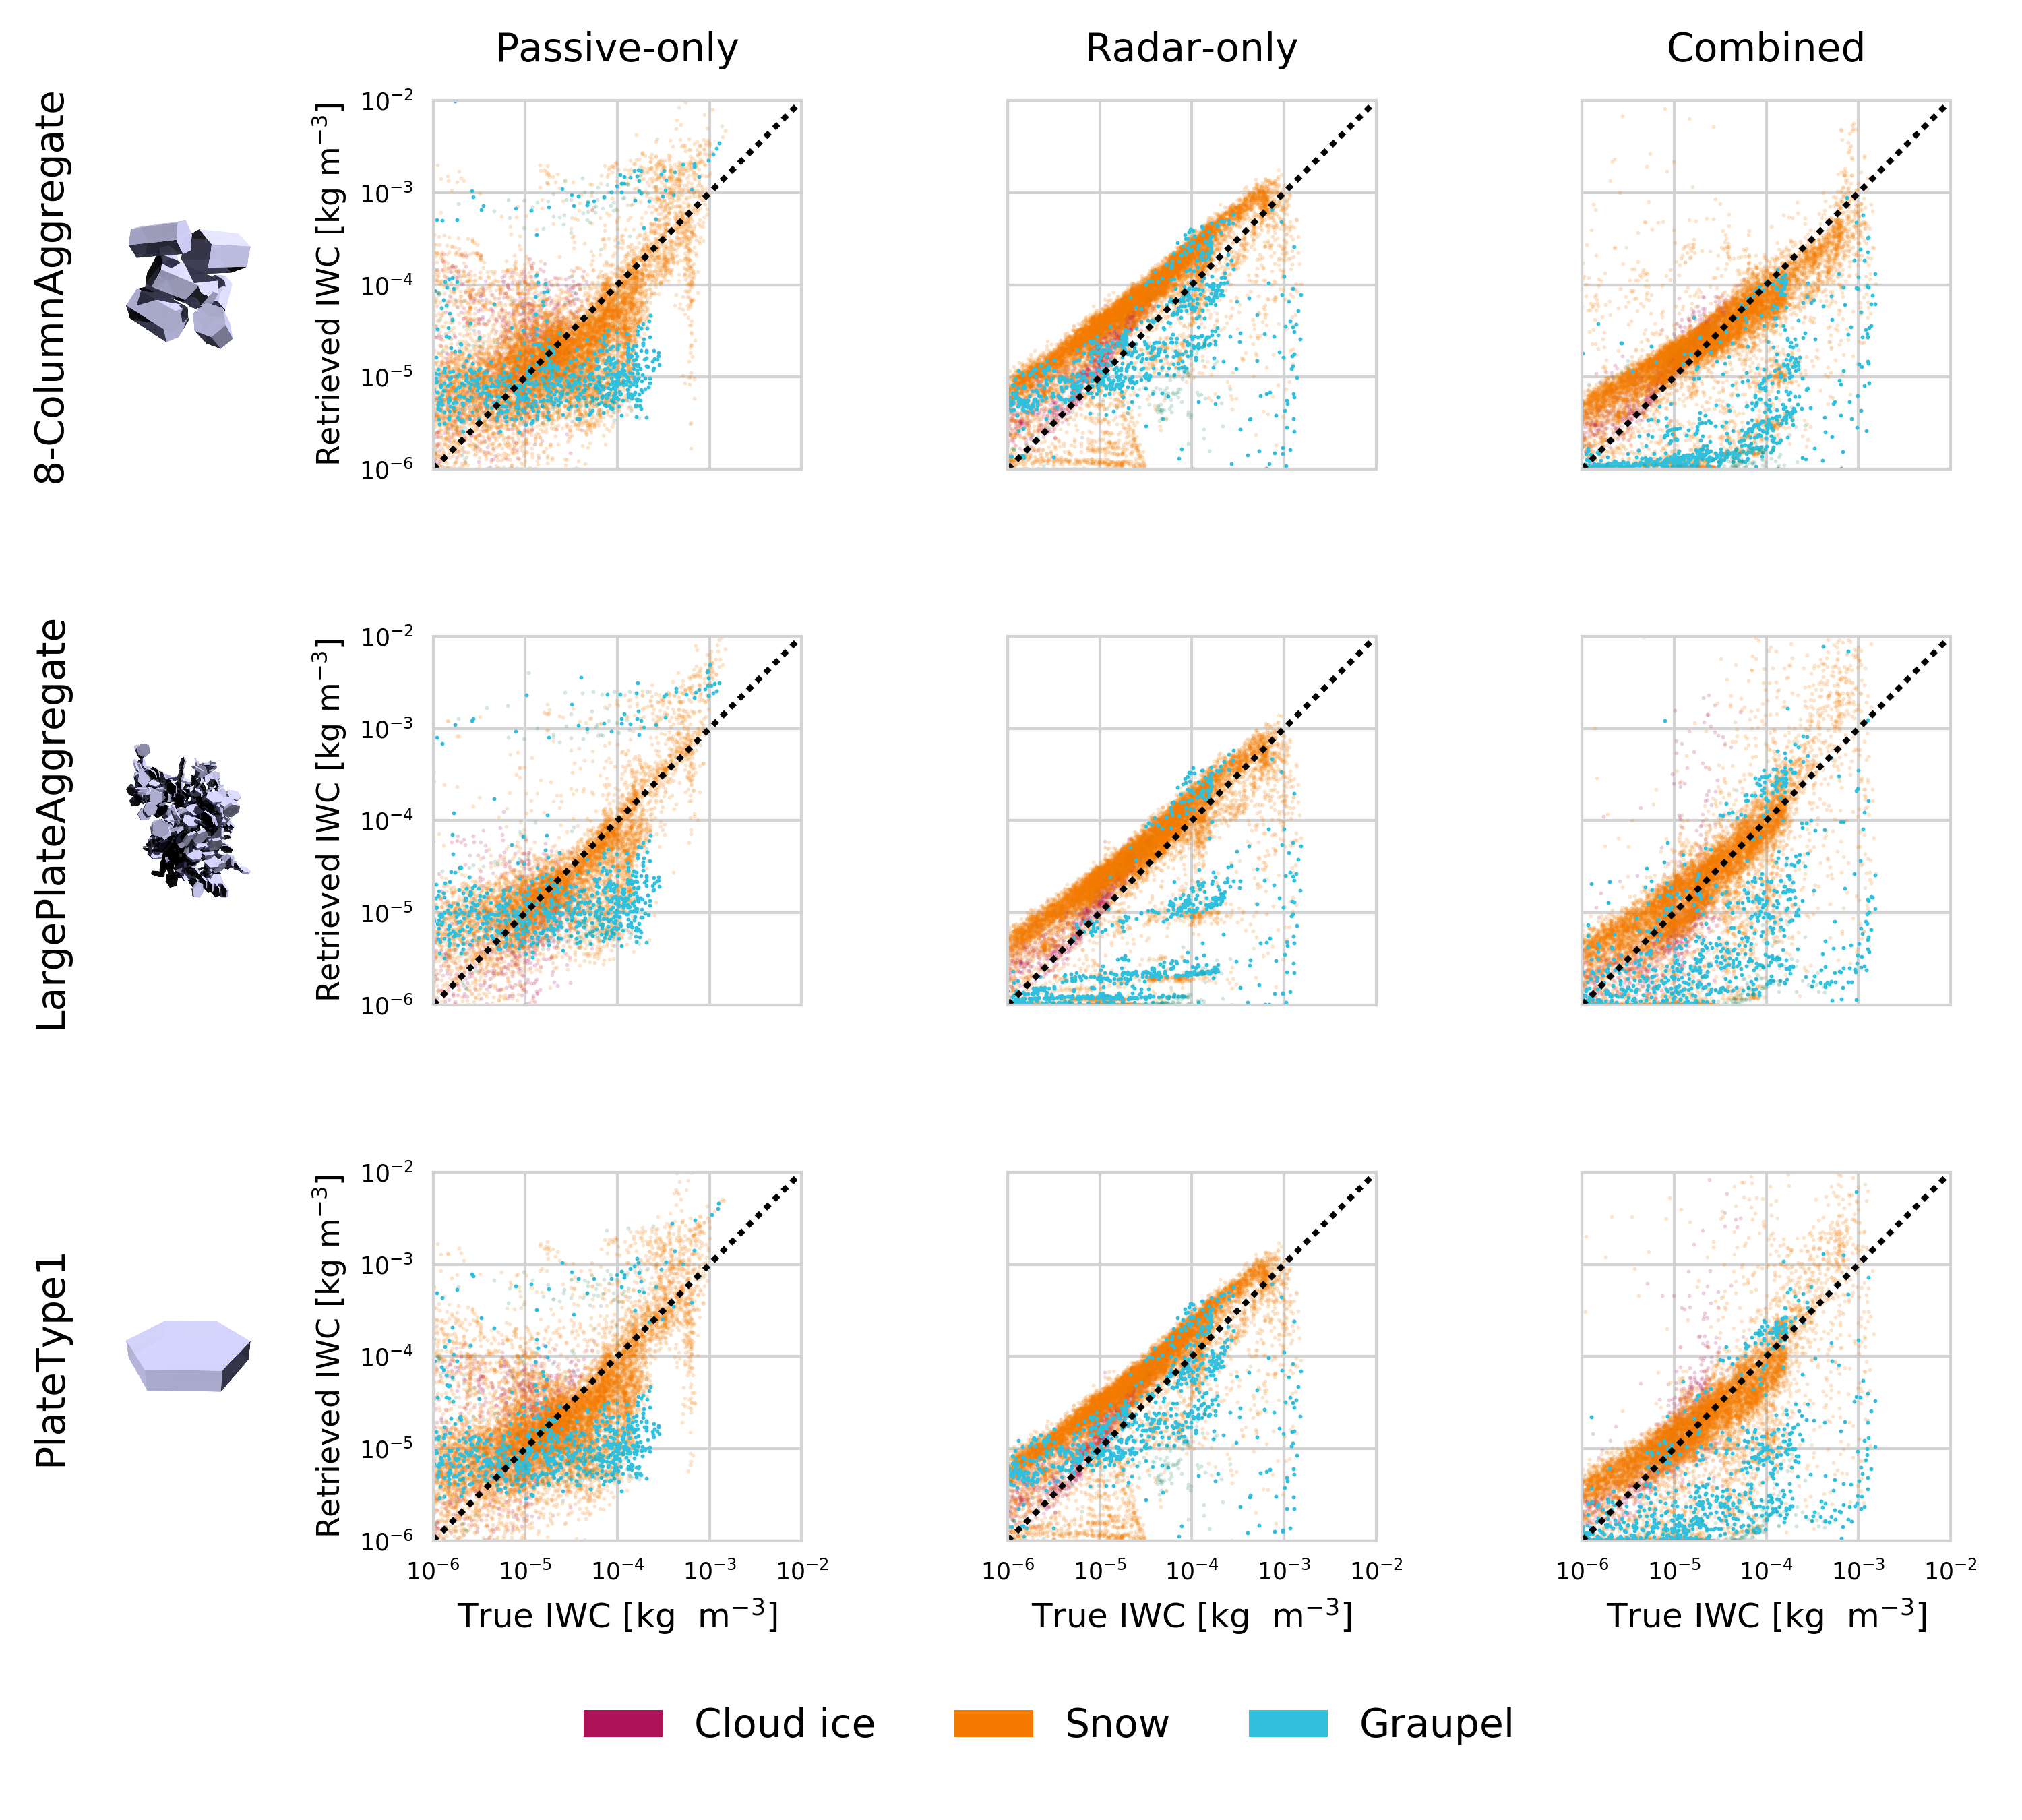
\includegraphics[width = 0.8\textwidth]{../plots/results_scatter_b_2}
\caption{IWC retrieval results for the remaining particle models. Panels
  are similar to Fig.~8 in the main article.}
\end{figure}
\clearpage

\subsection{Number densities}

\begin{figure}[!hbpt]
\centering
\includegraphics[width = 0.8\textwidth]{../plots/results_nd_b_GemCloudIce}
\caption{Reference and retrieved number densities of frozen hydrometeors for the
  GemCloudIce particle model. Panels are similar Fig.~12 in the main article.}
\end{figure}
\clearpage

\begin{figure}[!hbpt]
\centering
\includegraphics[width = 0.8\textwidth]{../plots/results_nd_b_GemSnow}
\caption{Reference and retrieved number densities of frozen hydrometeors for the
  GemSnow particle model. Panels are similar to Fig.~12 in the main article.}
\end{figure}
\clearpage

\begin{figure}[!hbpt]
\centering
\includegraphics[width = 0.8\textwidth]{../plots/results_nd_b_8-ColumnAggregate}
\caption{Reference and retrieved number densities of frozen hydrometeors for the
  8-ColumnAggregate particle model. Panels are similar Fig.~12 in the main article.}
\end{figure}
\clearpage

\begin{figure}[!hbpt]
\centering
\includegraphics[width = 0.8\textwidth]{../plots/results_nd_b_PlateType1}
\caption{Reference and retrieved number densities of frozen hydrometeors for the
  PlateType1 particle model. Panels are similar to Fig.~12 in the main article.}
\end{figure}
\clearpage

\begin{figure}[!hbpt]
\centering
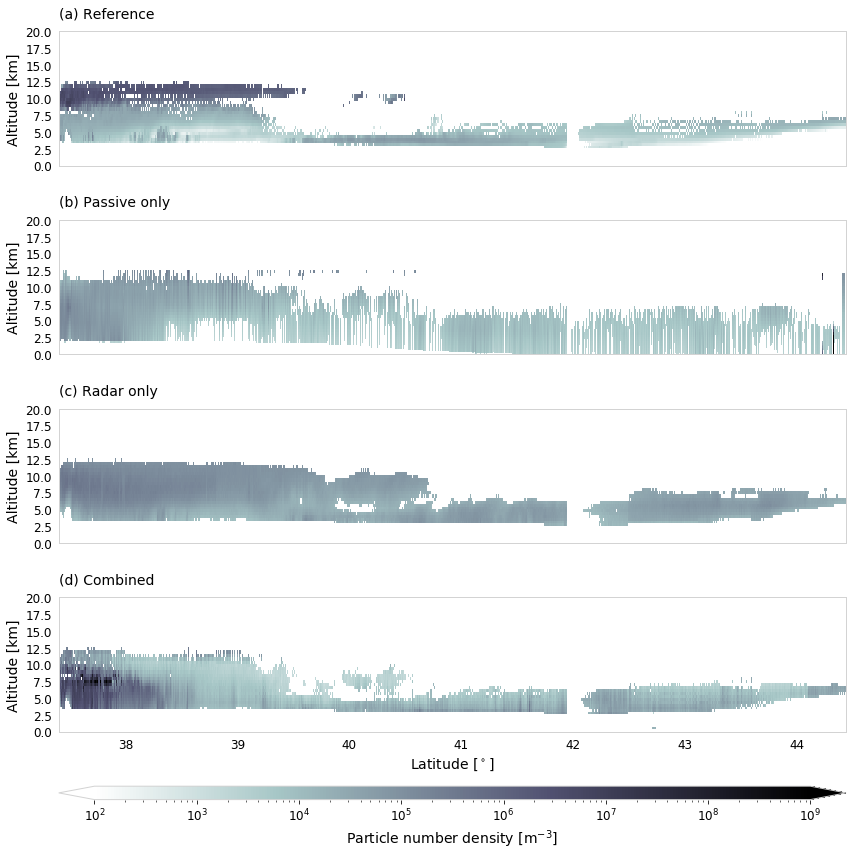
\includegraphics[width = 0.8\textwidth]{../plots/results_nd_b_LargePlateAggregate}
\caption{Reference and retrieved number densities of frozen hydrometeors for the
  LargePlateAggregate particle model. Panels are similar to Fig.~12 in the main article.}
\end{figure}
\clearpage

\begin{figure}[!hbpt]
\centering
\includegraphics[width = 0.8\textwidth]{../plots/results_nd_scatter_b}
\caption{Scatter plots of retrieved number densities for the remaining particle models. Panels
are similar to Fig.~13 in the main article.}
\end{figure}

\begin{figure}[!hbpt]
\centering
\includegraphics[width = 0.8\textwidth]{../plots/results_nd_scatter_b_1}
\caption{Scatter plots of retrieved number densities for the remaining particle models. Panels
are similar to Fig.~13 in the main article.}
\end{figure}
\clearpage

\subsection{LWC}

\begin{figure}[!hbpt]
\centering
\includegraphics[width = 0.8\textwidth]{../plots/results_cw_b_GemCloudIce}
\caption{Reference and retrieved LWC for the GemCloudIce particle model. Panels are similar to
Fig.~16 in the main article.}
\end{figure}
\clearpage

\begin{figure}[!hbpt]
\centering
\includegraphics[width = 0.8\textwidth]{../plots/results_cw_b_GemSnow}
\caption{Reference and retrieved LWC for the GemSnow particle model. Panels are similar to
Fig.~16 in the main article.}
\end{figure}
\clearpage

\begin{figure}[!hbpt]
\centering
\includegraphics[width = 0.8\textwidth]{../plots/results_cw_b_8-ColumnAggregate}
\caption{Reference and retrieved LWC for the 8-ColumnAggregate particle model. Panels are similar to
Fig.~16 in the main article.}
\end{figure}
\clearpage

\begin{figure}[!hbpt]
\centering
\includegraphics[width = 0.8\textwidth]{../plots/results_cw_b_PlateType1}
\caption{Reference and retrieved LWC for the PlateType1 particle model. Panels are similar to
Fig.~16 in the main article.}
\end{figure}
\clearpage
%% The following commands are for the statements about the availability of data sets and/or software code corresponding to the manuscript.
%% It is strongly recommended to make use of these sections in case data sets and/or software code have been part of your research the article is based on.

\noappendix       %% use this to mark the end of the appendix section
\end{document}
